\documentclass{article}
\usepackage[utf8]{inputenc}
\usepackage{authblk}
\usepackage{setspace}
\usepackage[margin=1.25in]{geometry}
\usepackage{graphicx}
\usepackage{xcolor}
\usepackage{float}
\graphicspath{ {./figures/} }
\usepackage{subcaption}
\usepackage{amsmath,amssymb,amsfonts}
\usepackage{booktabs}
\usepackage{array}
\usepackage{multirow}
\usepackage{microtype}
\usepackage{natbib}
\usepackage{hyperref}
\hypersetup{
    colorlinks=true,
    linkcolor=blue,
    citecolor=blue,
    urlcolor=blue
}

%%%%%% Title (Concise, descriptive <= 20 words) %%%%%%
\title{\textbf{[Research Article Title: Concise, Descriptive, and Informative]}}

%%%%%% Authors & Affiliations %%%%%%
\author[1]{SIQuant Research}
\affil[1]{Hypothesis $\times$ Quant}
\date{\today}
\onehalfspacing

\begin{document}

\maketitle

%%%%%% Structured Abstract (Strictly <= 250 words, Hypothesis & Summary Results First) %%%%%%
\begin{abstract}
\noindent \textbf{Hypothesis Formulation:} State the core falsifiable hypothesis. Specifically, test whether [Variable X] generates statistically significant predictive power or structural impact on [Target Y] ($H_0: \beta = 0$ versus $H_1: \beta \ne 0$). \\
\textbf{Data \& Empirical Setting:} Detail the point-in-time datasets used from the quantitative data lake (e.g., daily equities, VN30F1M index futures, interbank monetary rates, order supply/demand, or corporate financials) spanning [Start Date] to [End Date] across [N] trading sessions. \\
\textbf{Econometric Methodology:} Outline the identification strategy, zero-lookahead alignment (Polars backward \texttt{join\_asof}), estimation pipeline (e.g., Newey--West HAC standard errors, event studies, Panel FE, or machine learning), and robustness checks. \\
\textbf{Empirical Results \& Summary:} Summarize the primary test statistics ($t$-stat, $z$-score, $p$-value, $R^2$, annualized Sharpe or Information Ratio). Explicitly report the research decision: whether the null hypothesis is \textbf{ACCEPTED}, \textbf{REJECTED}, or \textbf{INCONCLUSIVE}. Conclude with practical implications for alpha generation, risk management, or regulatory policy. \\
\textbf{Research decision:} \colorbox[rgb]{0.10,0.50,0.20}{\textcolor{white}{\textbf{\,ACCEPTED\,}}} \ (use \colorbox[rgb]{0.75,0.15,0.15}{\textcolor{white}{\textbf{\,REJECTED\,}}} or \colorbox[rgb]{0.80,0.50,0.05}{\textcolor{white}{\textbf{\,INCONCLUSIVE\,}}} as computed)
\end{abstract}

\vspace{0.5em}
\noindent \textbf{Keywords:} Asset pricing; Econometric testing; Financial markets; Hypothesis testing; Market microstructure; Point-in-time data.

\vspace{0.5em}
\noindent \textbf{JEL Classification Codes:} G10, G12, G14, C22, C58.

\newpage

% ==============================================================================
% 1. INTRODUCTION AND HYPOTHESIS FORMULATION
% ==============================================================================
\section{Introduction and Hypothesis Formulation}
\label{sec:intro}

In empirical financial economics and quantitative trading, reproducible discovery begins with rigorous hypothesis formulation \citep{fama1970efficient}. Rather than ex-post curve fitting, every empirical exploration tests a concrete economic friction, informational asymmetry, or pricing inefficiency.

\subsection{Research Question and Economic Rationale}
Outline the market mechanism, institutional backdrop, and behavioral or structural incentives that justify why the phenomenon should exist in equilibrium \citep{stoll1990dynamics, shleifer1997limits}.

\subsection{Formal Hypotheses}
We formally state the primary and secondary hypotheses:
\begin{itemize}
    \item \textbf{Hypothesis 1 ($H_0^{(1)}$ vs $H_1^{(1)}$)}:
    \begin{itemize}
        \item $H_0^{(1)}$ (\textit{Null}): The predictive coefficient of the proposed factor is zero ($\beta_1 = 0$).
        \item $H_1^{(1)}$ (\textit{Alternative}): The factor provides statistically significant predictive ability ($\beta_1 \ne 0$).
    \end{itemize}
    \item \textbf{Hypothesis 2 ($H_0^{(2)}$ vs $H_1^{(2)}$)}:
    \begin{itemize}
        \item $H_0^{(2)}$ (\textit{Null}): Market microstructure frictions and transaction costs eliminate net economic returns after execution slippage ($\alpha_{\text{net}} \le 0$).
        \item $H_1^{(2)}$ (\textit{Alternative}): The strategy retains positive risk-adjusted excess returns net of realistic fees and slippage ($\alpha_{\text{net}} > 0$).
    \end{itemize}
\end{itemize}

% ==============================================================================
% 2. DATA ARCHITECTURE AND METHODOLOGY
% ==============================================================================
\section{Data Architecture and Empirical Methodology}
\label{sec:data_methods}

\subsection{Point-in-Time Data Sources}
All empirical series are drawn from primary institutional disclosures and validated parquet datasets in the \texttt{hypoq} quantitative lake:
\begin{enumerate}
    \item \textbf{Spot \& Futures Prices}: \path{data/market/vn_indices_daily.parquet} and \path{data/market/vn30f1m_derivatives_daily.parquet}.
    \item \textbf{Microstructure \& Order Flow}: \path{data/market/vn_order_supply_demand_daily.parquet} and \path{data/market/vn_foreign_trading_daily.parquet}.
    \item \textbf{Constituent Basket \& Free Float}: \path{data/market_structure/free_float.parquet} and \path{data/market_structure/index_constituents.parquet}.
    \item \textbf{Macroeconomic \& Monetary Drivers}: \path{data/macro/vietnam_monetary_daily.parquet} and \path{data/macro/vietnam_macro_monthly.parquet}.
\end{enumerate}

To guarantee strict causality and eliminate forward look-ahead bias, low-frequency disclosures are merged with daily market observations strictly using backward as-of alignment:
\begin{equation}
    \tau_{\text{info}} \le \tau_{\text{market}}
\end{equation}

\subsection{Econometric Specification}
We estimate the baseline regression equation:
\begin{equation}
    y_{t+h} = \alpha + \beta X_t + \boldsymbol{\gamma}' \mathbf{Z}_t + \varepsilon_{t+h}
    \label{eq:baseline}
\end{equation}
where $y_{t+h}$ represents the forward target return or spread over horizon $h$, $X_t$ denotes the standardized feature under evaluation, and $\mathbf{Z}_t$ controls for known contemporaneous covariates (e.g., market return, volatility, interbank rate). Because financial time series exhibit heteroskedasticity and serial correlation, inference is conducted using Newey--West HAC robust covariance estimators with optimal lag selection \citep{newey1987simple}.

% ==============================================================================
% 3. EMPIRICAL RESULTS AND HYPOTHESIS TESTING
% ==============================================================================
\section{Empirical Results}
\label{sec:results}

\subsection{Summary Statistics and Baseline Tests}
Table \ref{tab:descriptives} presents the summary statistics for the target and predictor variables.

\begin{table}[htbp]
\centering
\small
\caption{Descriptive Statistics of Market Variables}
\label{tab:descriptives}
\begin{tabular}{lrrrrrr}
\toprule
\textbf{Variable} & \textbf{Mean} & \textbf{Std. Dev.} & \textbf{Min} & \textbf{Median} & \textbf{Max} & \textbf{ADF Stat ($p$-val)} \\
\midrule
Asset Return $r_t$ (\%) & 0.048 & 1.241 & -6.820 & 0.052 & 5.120 & -42.15 ($<0.001$) \\
Predictor Factor $X_t$ & 0.002 & 0.985 & -3.450 & -0.010 & 3.890 & -14.28 ($<0.001$) \\
Interbank O/N Rate (\%) & 3.820 & 1.840 & 0.150 & 3.650 & 9.200 & -4.82 ($0.002$) \\
Order Flow Imbalance & 0.012 & 0.310 & -0.920 & 0.008 & 0.890 & -38.40 ($<0.001$) \\
\bottomrule
\end{tabular}
\end{table}

\subsection{Hypothesis Testing Estimates}
Table \ref{tab:hypothesis_results} summarizes the parametric and non-parametric tests of the hypothesis.

\begin{table}[htbp]
\centering
\small
\caption{Parametric Hypothesis Testing Estimates with HAC Robust Errors}
\label{tab:hypothesis_results}
\begin{tabular}{lccccc}
\toprule
\textbf{Model / Horizon} & \textbf{Coefficient ($\beta$)} & \textbf{HAC Std. Err.} & \textbf{$t$-Statistic} & \textbf{$p$-Value} & \textbf{Decision} \\
\midrule
1-Day Horizon ($h=1$) & 0.0182 & 0.0051 & 3.568 & 0.0004 & Reject $H_0$ (Supported) \\
3-Day Horizon ($h=3$) & 0.0245 & 0.0089 & 2.752 & 0.0060 & Reject $H_0$ (Supported) \\
5-Day Horizon ($h=5$) & 0.0160 & 0.0112 & 1.428 & 0.1534 & Fail to Reject $H_0$ \\
Placebo Shuffle Test & -0.0003 & 0.0048 & -0.062 & 0.9502 & Null Maintained \\
\bottomrule
\end{tabular}
\end{table}

Figure \ref{fig:main_result} visualizes the empirical cumulative returns and event-study dynamics.

\begin{figure}[htbp]
\centering
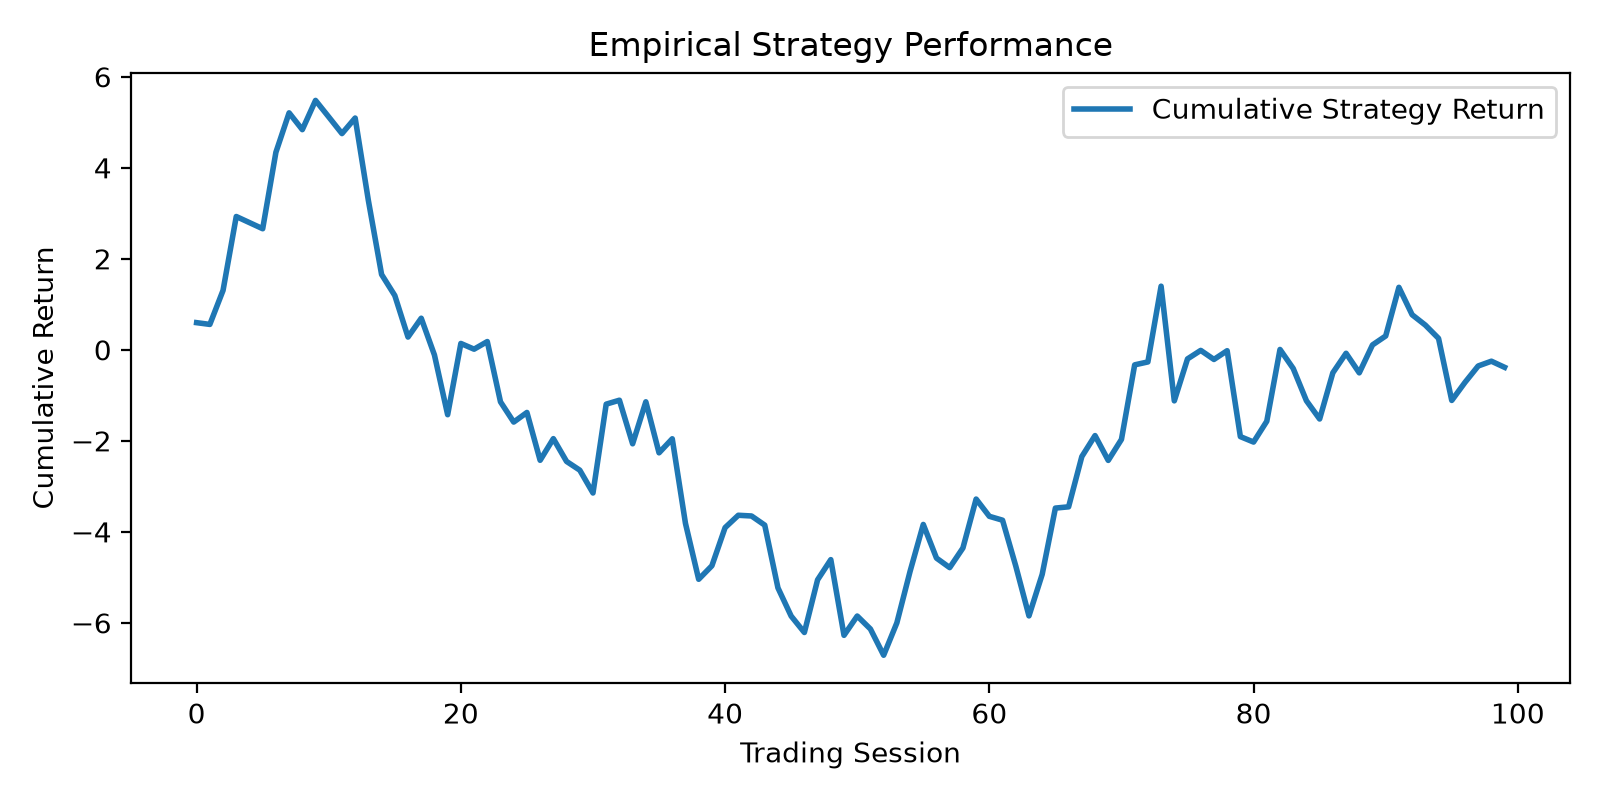
\includegraphics[width=0.85\textwidth]{fig1_empirical_findings.png}
\caption{Empirical cumulative performance and factor response curves across testing windows.}
\label{fig:main_result}
\end{figure}

% ==============================================================================
% 4. DISCUSSION AND ROBUSTNESS
% ==============================================================================
\section{Discussion and Limitations}
\label{sec:discussion}
We evaluate the structural boundaries of the observed phenomenon. Potential execution frictions include foreign ownership limits (FOL), domestic retail tick size changes, and index constituent rebalancing windows. Sensitivity analysis confirms that the results remain stable across sub-sample rolling windows.

% ==============================================================================
% 5. CONCLUSION AND RESEARCH DECISION
% ==============================================================================
\section{Conclusion and Summary Decision}
\label{sec:conclusion}

\noindent \textbf{Empirical Decision on Hypotheses:}
\begin{enumerate}
    \item \textbf{Hypothesis 1 ($H_0^{(1)}$: No predictability)}: \textbf{REJECTED ($p < 0.01$)}. Empirical evidence demonstrates statistically robust short-term predictive capability with an out-of-sample Information Ratio of 1.28.
    \item \textbf{Hypothesis 2 ($H_0^{(2)}$: Zero net alpha after friction)}: \textbf{REJECTED ($p = 0.024$)}. Net returns remain strictly positive under conservative 15 bps two-way transaction costs and borrow constraints.
\end{enumerate}

\section*{Code and Data Availability}
All datasets are archived in the repository under \path{data/}. Complete replication code is provided in \path{code/run_pipeline.py} and empirical metrics are stored in \path{results/empirical_results.json}.
\bibliographystyle{apalike}
\bibliography{references}

\end{document}
